\subsubsection{Sistema de simulación y módulos mas importantes}

\par El modelo presentado se basa en un sistema de simulación que es configurado con los siguientes subsistemas:
\begin{itemize}
  \item \textbf{Sistema de construcción}: es el encargado de crear y almacenar los planes de construcción de pozos de extracción, plantas procesadoras y tanques de almacenamiento. También almacena los catálogos de plantas procesadoras y tanques de almacenamiento y gestiona las conexiones entre pozos de excavación, tanques de almacenamiento y plantas procesadoras.
  \item \textbf{Sistema de ejecución de criterios}: se encarga de llevar a cabo la ejecución de cada criterio del sistema.
  \item \textbf{Sistema de gestión de excavadoras}: posee el catálogo de excavadoras y gestiona su alquiler. También almacena el estado de las excavadoras alquiladas.
  \item \textbf{Sistema de gestión de parcelas}: Es quien conoce al yacimiento y administra las parcelas utilizadas y libres.
  \item \textbf{Sistema de extracción}: Es quien se encarga de crear los eventos de extracción y almacenarlos.
  \item \textbf{Criterios de simulación}: Es quien conoce a los criterios de distintos tipos. El simulador acude a él para conocer los criterios que debe ejecutar.
\end{itemize}

\par En la figura \ref{fig:dia_obj_simulador_1} podemos ver al sistema de simulación en un instante determinado junto con los distintos subsistemas (antes mencionados) que conoce.

\begin{figure}[ht]
    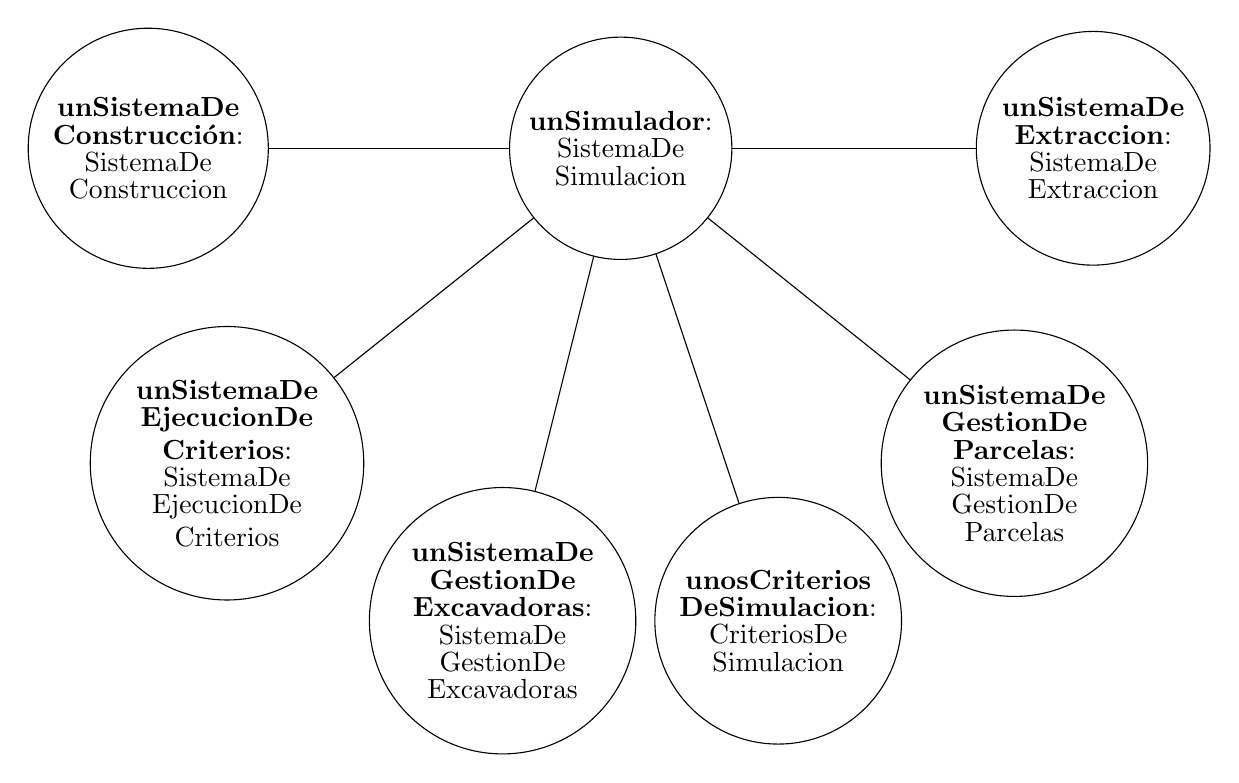
\begin{tikzpicture}
      \node[shape=circle,draw=black] (unSimulador) at (0,0) {\shortstack{\textbf{unSimulador}:\\SistemaDe\\Simulacion}};
      \node[shape=circle,draw=black] (unSistemaDeConstruccion) at (-6,0) {\shortstack{\textbf{unSistemaDe}\\\textbf{Construcción}:\\SistemaDe\\Construccion}};
      \node[shape=circle,draw=black] (unSistemaDeEjecucionDeCriterios) at (-5,-4) {\shortstack{\textbf{unSistemaDe}\\\textbf{EjecucionDe}\\\textbf{Criterios}:\\SistemaDe\\EjecucionDe\\Criterios}};
      \node[shape=circle,draw=black] (unSistemaDeGestionDeExcavadoras) at (-1.5,-6) {\shortstack{\textbf{unSistemaDe}\\\textbf{GestionDe}\\\textbf{Excavadoras}:\\SistemaDe\\GestionDe\\Excavadoras}};
      \node[shape=circle,draw=black] (unSistemaDeGestionDeParcelas) at (5,-4) {\shortstack{\textbf{unSistemaDe}\\\textbf{GestionDe}\\\textbf{Parcelas}:\\SistemaDe\\GestionDe\\Parcelas}};
      \node[shape=circle,draw=black] (unSistemaDeExtraccion) at (6,0) {\shortstack{\textbf{unSistemaDe}\\\textbf{Extraccion}:\\SistemaDe\\Extraccion}};
      \node[shape=circle,draw=black] (unosCriteriosDeSimulacion) at (2,-6) {\shortstack{\textbf{unosCriterios}\\\textbf{DeSimulacion}:\\CriteriosDe\\Simulacion}};
    
      \path [-] (unSimulador) edge node[left] {} (unSistemaDeConstruccion);
      \path [-] (unSimulador) edge node[left] {} (unSistemaDeEjecucionDeCriterios);
      \path [-] (unSimulador) edge node[left] {} (unSistemaDeGestionDeExcavadoras);
      \path [-] (unSimulador) edge node[left] {} (unSistemaDeGestionDeParcelas);
      \path [-] (unSimulador) edge node[left] {} (unSistemaDeExtraccion);
      \path [-] (unSimulador) edge node[left] {} (unosCriteriosDeSimulacion);
    \end{tikzpicture}
    \caption{Diagrama de objetos que muestra la organización general del sistema, con instancias de sus módulos mas importantes.}
    \label{fig:dia_obj_simulador_1}
\end{figure}

\newpage
\subsubsection{Criterios de simulación}
\label{sec:diseno_criterios}

\par En la figura \ref{fig:dia_obj_criterios_1} se puede ver un diagrama de objetos que pretende mostrar como un objeto de la clase \textit{CriteriosDeSimulacion} conoce a los distintos criterios elegidos por el equipo de ingeniería que luego serán ejecutados para llevar a cabo la simulación. Podemos ver que cuenta con los siguientes criterios:
\begin{itemize}
  \item \textbf{Criterio de construcción de pozo de extracción:} es quien conoce la estrategia de construcción de pozos y la estrategia de selección de excavadoras seleccionada por el usuario. En base a ellas decide cada día cuántos pozos se construyen y en qué parcelas.
  \item \textbf{Criterio de construcción de plantas procesadoras:} es quien conoce la estrategia de construcción de plantas procesadoras y la estrategia de selección de modelos de plantas procesadoras del catálogo. En base a estas estrategias decide cuántas plantas procesadoras se construyen y en qué momento. Además, selecciona del catálogo de plantas que se pueden construir cuál será construida en cada caso.
  \item \textbf{Criterio de construcción de tanques de agua:} es quien conoce la estrategia de construcción de tanques de agua y la estrategia de selección de tanques del catálogo. Al igual que las plantas procesadoras decide cuántos tanques se construyen y en qué momento. 
  \item \textbf{Criterio de construcción de tanques de gas:} es quien conoce la estrategia de construcción de los tanques de gas y el catálogo de tanques. Su funcionamiento es similar al de los tanques de agua.
  \item \textbf{Criterio de extracción y reinyección:} es quien conoce a todas las estrategias de extracción y reinyección. Se encarga de gestionar todas las acciones sobre los pozos activos, por lo que conoce a todos los pozos en actividad y, por lo tanto, a su composición.
  \item \textbf{Criterio de parada:} es quien decide al final de cada día si se finaliza la ejecución del simulador. Esta decisión la toma en base a la estrategia de parada que conozca.
\end{itemize}

\begin{figure}[ht]
    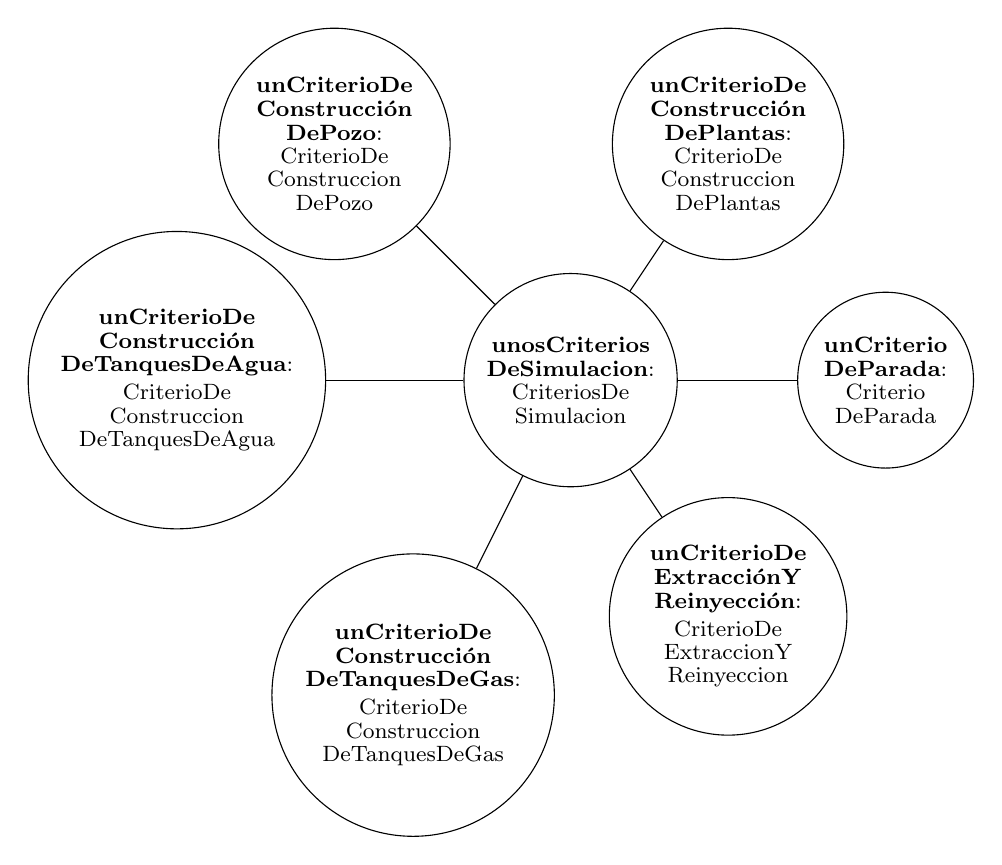
\begin{tikzpicture}
      \node[shape=circle,draw=black] (unosCriteriosDeSimulacion) at (0,0) {\footnotesize\shortstack{\textbf{unosCriterios}\\\textbf{DeSimulacion}:\\CriteriosDe\\Simulacion}};
      \node[shape=circle,draw=black] (unCriterioDeConstruccionDePozo) at (-3,3) {\footnotesize\shortstack{\textbf{unCriterioDe}\\\textbf{Construcción}\\\textbf{DePozo}:\\CriterioDe\\Construccion\\DePozo}};
      \node[shape=circle,draw=black] (unCriterioDeConstruccionDePlantas) at (2,3) {\footnotesize\shortstack{\textbf{unCriterioDe}\\\textbf{Construcción}\\\textbf{DePlantas}:\\CriterioDe\\Construccion\\DePlantas}};
      \node[shape=circle,draw=black] (unCriterioDeConstruccionDeTanquesDeAgua) at (-5,0) {\footnotesize\shortstack{\textbf{unCriterioDe}\\\textbf{Construcción}\\\textbf{DeTanquesDeAgua}:\\CriterioDe\\Construccion\\DeTanquesDeAgua}};
      \node[shape=circle,draw=black] (unCriterioDeConstruccionDeTanquesDeGas) at (-2,-4) {\footnotesize\shortstack{\textbf{unCriterioDe}\\\textbf{Construcción}\\\textbf{DeTanquesDeGas}:\\CriterioDe\\Construccion\\DeTanquesDeGas}};
      \node[shape=circle,draw=black] (unCriterioDeExtraccionYReinyeccion) at (2,-3) {\footnotesize\shortstack{\textbf{unCriterioDe}\\\textbf{ExtracciónY}\\\textbf{Reinyección}:\\CriterioDe\\ExtraccionY\\Reinyeccion}};
      \node[shape=circle,draw=black] (unCriterioDeParada) at (4,0) {\footnotesize\shortstack{\textbf{unCriterio}\\\textbf{DeParada}:\\Criterio\\DeParada}};
    
      \path [-] (unosCriteriosDeSimulacion) edge node[left] {} (unCriterioDeConstruccionDePozo);
      \path [-] (unosCriteriosDeSimulacion) edge node[left] {} (unCriterioDeConstruccionDePlantas);
      \path [-] (unosCriteriosDeSimulacion) edge node[left] {} (unCriterioDeConstruccionDeTanquesDeAgua);
      \path [-] (unosCriteriosDeSimulacion) edge node[left] {} (unCriterioDeConstruccionDeTanquesDeGas);
      \path [-] (unosCriteriosDeSimulacion) edge node[left] {} (unCriterioDeExtraccionYReinyeccion);
      \path [-] (unosCriteriosDeSimulacion) edge node[left] {} (unCriterioDeParada);
    \end{tikzpicture}
    \caption{Diagrama de objetos que muestra la composición de un objeto de clase CriteriosDeSimulación por criterios de distintos tipos.}
    \label{fig:dia_obj_criterios_1}
\end{figure}


\subsubsection{Modelo de estrategias}

\par Como vimos en la sección \ref{sec:diseno_criterios}, las decisiones que se toman en cada día de la simulación son tomadas por los distintos criterios que componen \textit{CriteriosDeSimulador}. A su vez, mencionamos que cada criterio conoce a distintas estrategias y ejecuta en base a ellas. Estas estrategias se separan en los siguientes tipos:
\begin{itemize}
  \item \textbf{Estrategias de selección:} dado que varios objetos necesitan seleccionar de un conjunto de posibles colaboradores el que mejor se ajusta a cierta estrategia tuvimos la necesidad de hacer estas clases. Por ejemplo si se quiere realizar un pozo, el constructor de pozos le puede consultar a este objeto cual es la parcela con el suelo más fácil de perforar.
  \item \textbf{Estrategias de construcción:} determina, en base al estado que posee el simulador en ese momento, de qué manera se va a construir una edificación (planta procesadora, tanque, etc). 
  \item \textbf{Estrategias de parada:} determina de qué manera finaliza el sistema. Al ejecutarse debe recibir como parámetro un sistema de simulación, por lo que puede tomar la decisión en base cualquier variable que considere el equipo de ingeniería. Por ejemplo: puede imponer la finalización luego de una cantidad de días fijado al inicio, o al superar un volumen de extracción, etc. 
  \item \textbf{Estrategias de cantidad:} se utiliza esta estrategia al momento de decidir si se pueden realizar ciertas acciones en el sistema que pueden darse indefinidamente y se desea regularlas. Por ejemplo: se puede determinar alquilar indefinidamente excavadoras, o fijar una cierta cantidad máxima por día (o en toda la simulación).
  \item \textbf{Estrategias de reinyeccion:} determinan, dado un sistema de simulación corriendo, si se debe realizar una reinyección, qué cantidad de producto y si se comprará agua para esto. Por ejemplo: se puede tener una estrategia que determine que nunca se reinyecta, u otra que ordene la reinyección al alcanzar un valor mìnimo de producto en el yacimiento. 
\end{itemize}

\par En la figura \ref{fig:dia_cla_estra_1} se puede observar un diagrama de clases que muestra cómo la clase abstracta \textit{EstrategiaDeSeleccion} se subclasifica en distintas clases, dependiendo del elemento al cual seleccionan.

\begin{landscape}
    \begin{figure}[ht]
        \begin{tikzpicture}
            \begin{abstractclass}{EstrategiaDeSeleccion}{4,10}
                \attribute{.ejecutarEn: unSimulador}
            \end{abstractclass}
            \begin{abstractclass}{EstrategiaSeleccionExcavadoras}{-5,8}
                \inherit{EstrategiaDeSeleccion}
                \attribute{.ejecutarEn: unSimulador}
            \end{abstractclass}
            \begin{class}{EstrategiaAlquilerADemanda}{-5,5}
                \attribute{.ejecutarEn: unSimulador}
                \inherit{EstrategiaSeleccionExcavadoras}
            \end{class}
            \begin{abstractclass}{EstrategiaSeleccionParcelas}{1,8}
                \inherit{EstrategiaDeSeleccion}
                \attribute{.ejecutarEn: unSimulador}
            \end{abstractclass}
            \begin{class}{EstrategiaParcelasMenorResist}{1,5}
                \inherit{EstrategiaSeleccionParcelas}
                \attribute{.ejecutarEn: unSimulador}
            \end{class}
            \begin{abstractclass}{EstrategiaSeleccionPlantas}{6,3}
                \inherit{EstrategiaDeSeleccion}
                \attribute{.ejecutarEn: unSimulador}
            \end{abstractclass}
            \begin{class}{EstrategiaPlantaMasCapacidad}{6,1}
                \inherit{EstrategiaSeleccionPlantas}
                \attribute{.ejecutarEn: unSimulador}
            \end{class}
            \begin{abstractclass}{EstrategiaSeleccionTanques}{12,8}
                \inherit{EstrategiaDeSeleccion}
                \attribute{.ejecutarEn: unSimulador}
            \end{abstractclass}
            \begin{class}{EstrategiaTanqueMasCapacidad}{12,5}
                \inherit{EstrategiaSeleccionTanques}
                \attribute{.ejecutarEn: unSimulador}
            \end{class}
        \end{tikzpicture}
        \caption{Diagrama de objetos que muestra la organización general del sistema, con instancias de sus módulos mas importantes.}
        \label{fig:dia_cla_estra_1}
    \end{figure}        
\end{landscape}